\section{Case Studies}
\label{sec:cases}

This section discusses our experience in evaluating prior prototypes under
a wider range of settings, including both correctness and performance issues.
We try our best to fix these issues, but due to time constraints and the nature of debugging, we
are only able to fix a subset of them. Significant design-level changes are also out of the scope
of this paper.

\subsection{Correctness Issues}

\paragraph{Configuration issues.}

Many systems have hard-coded configuration parameters, which prevent extensive evaluation.

\begin{itemize}[leftmargin=*]

    \vspace{-.05in}
    \item Fixed memory allocation. Silo, Cicada, DrTM, and GAM allocate a fixed
    amount of memory. As a result, they fail if the experiments load more data,
    even if there is enough physical memory. Fixing these issues is often not
    as simple as changing a value, since some systems need to allocate memory 
    separately for different types of data 
    (e.g., Silo allocates a memory region for its underlying B\textsuperscript{+} tree nodes and database records, 
    plus a buffer region for each thread), and we had to manually tune the size of each part to
    maximize the total amount of data they can support.
    
    \vspace{-.05in}
    \item Fixed thread/warehouse ratio. DrTM assumes the
    number of threads is equal to the number of warehouses. When we test with
    more warehouses, this leads to significant performance degradation.
    We fixed this issue by modifying DrTM source
    code to allow a thread to access more than one warehouse. Janus
    has the same constraint but due to time constraints, we have not fixed it.
    
    \vspace{-.05in}
    \item Too many open files. In Janus, we met a problem that the server processes
    fail to start when we start many servers. After debugging, we find the root cause
    is that, in Janus, every server thread needs to open a socket to every other server
    thread, so when starting many servers, the number of sockets on one server becomes larger
    than the default maximal number of open files allowed by Linux. While fixing this issue is simple (i.e.,
    enlarge the maximal number of open files), such all-to-all socket creation may create
    scalability problems in a large deployment.
    
    \vspace{-.05in}
    \item Inappropriate timeout values. Many systems use timeout for different purposes, like
    detecting whether a node has failed or whether an experiment has failed. Under a new
    setting, however, the default timeout value sometimes becomes inappropriate, causing phenomena
    like a running experiment or a healthy node getting killed. We manually tune
    the timeout value when the default one does not work.
    
    \vspace{-.05in}
    \item Limit on message size. HERD relies on the RDMA inlining feature to improve
    performance, and this feature usually only allows messages smaller than 512B.
    This problem is admitted in the HERD paper, and a complete solution would be to design
    additional communication paths for larger messages. Since the additional path does not affect
    messages using the inlining feature, we have not implemented it.
    
\end{itemize}

Besides, a number of systems do not implement all the parameters we have tried.
For example,
%Cicada does not allow to tune the rate of cross warehouse transactions on TPC-C; 
TAPIR
uses one thread per server, so we cannot tune the number of threads; many systems can only
support two types of transactions in TPC-C. Fixing these issues requires much more effort
and thus is out of the scope of this paper. Furthermore, some issues are caused by the inherent limitation of these
works (e.g., in TPC-C, \emph{New-Order} and \emph{Payment} do not need range queries
but the other three types need).

We make the following observations and suggestions: 1) it is often not hard to find
a workaround after we know the root cause,
%(e.g., fixed memory allocation, limit on message size),
but it sometimes takes longer to diagnose the root cause since the error messages often do not directly point to the root cause.
Performing an extensive evaluation would help the researcher to identify and fix these issues,
and help later works to compare to this work. 2) A fundamental solution to these problems, however,
probably requires more thoughts (e.g., adaptive memory allocation, adaptive timeout, etc) and 
could be a research problem.
%3) If our community plans to encourage extensive evaluation, then we should have a consensus
%about which parameters should be tuned, at least for those very popular benchmarks, so that different
%works can be compared under the same settings.

\begin{figure*}[ht]
    \centering
     \begin{subfigure}[t]{0.45\textwidth}
         \centering
         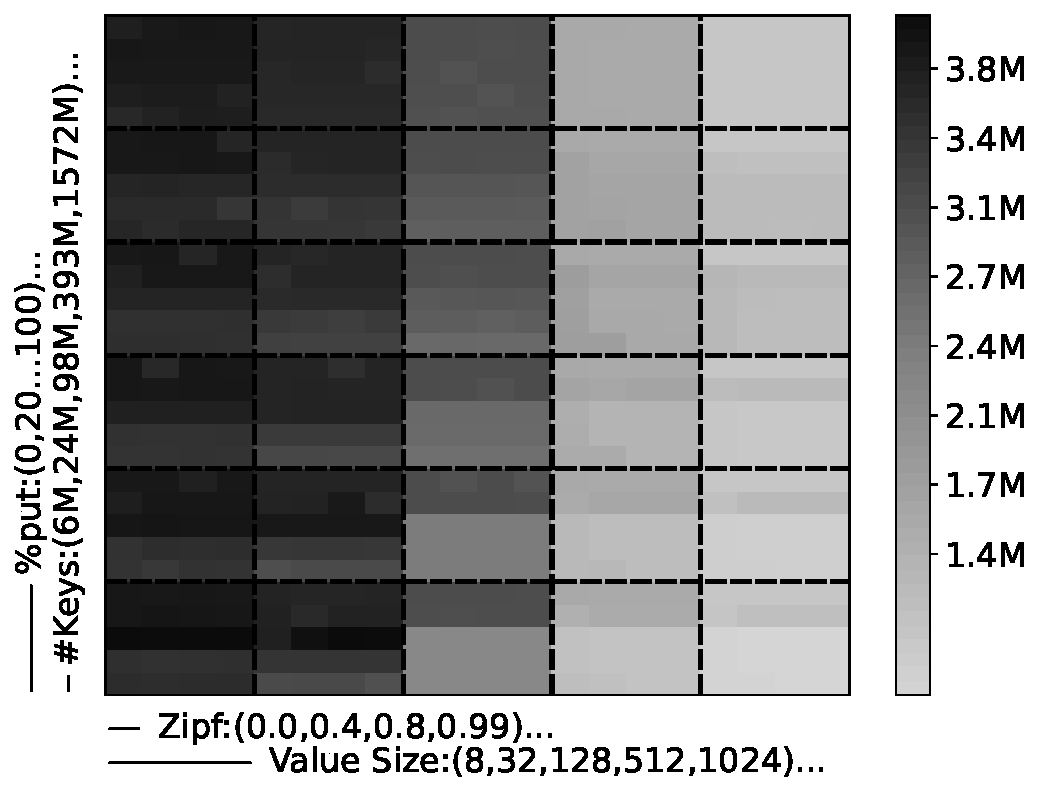
\includegraphics[width=\textwidth]{fig/herd/herd_ycsb.pdf}
         \caption{Per core throughput of HERD YCSB.}
         \label{fig:herd-throughput}
     \end{subfigure}
~
     \begin{subfigure}[t]{0.45\textwidth}
         \centering
         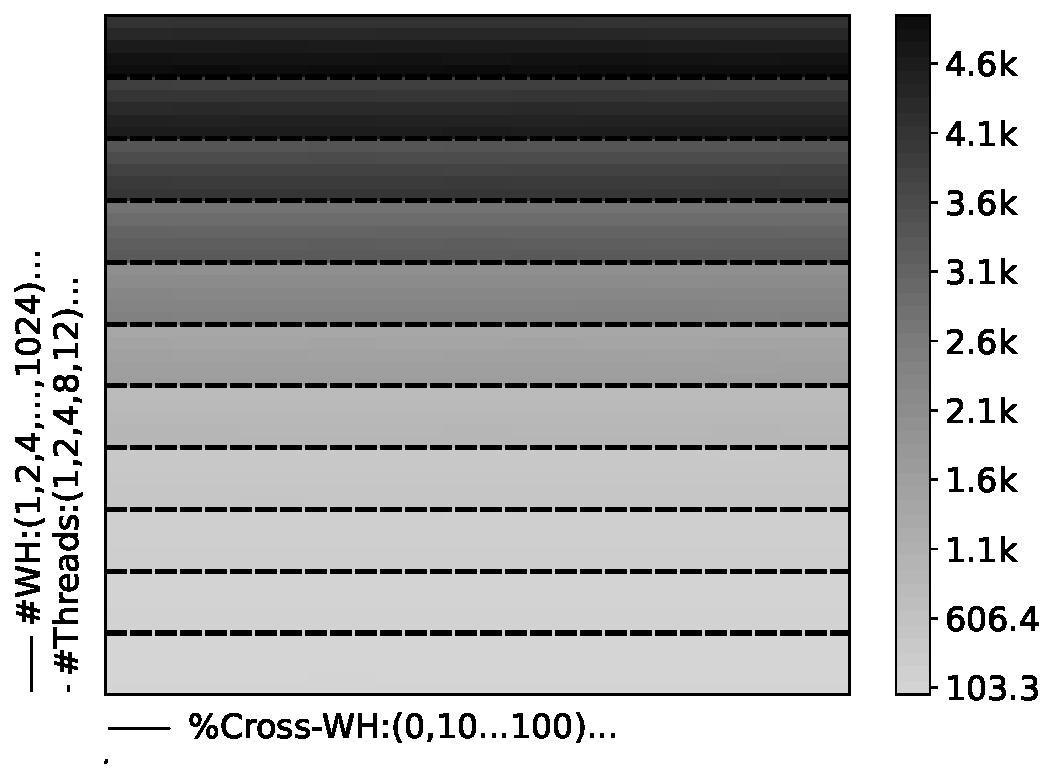
\includegraphics[width=\textwidth]{fig/aria/Aria_tpcc.pdf}
         \caption{Per core throughput of Aria TPC-C.}
         \label{fig:aria-throughput}
     \end{subfigure}
     
    \begin{subfigure}[t]{0.45\textwidth}
         \centering
         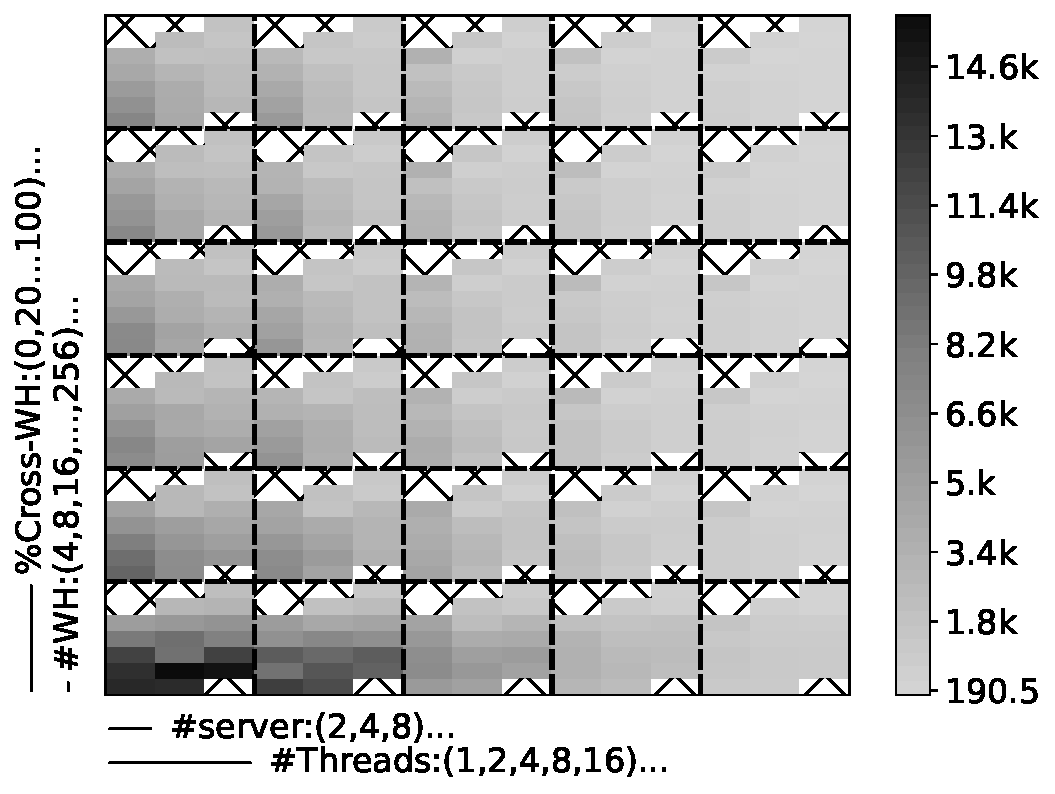
\includegraphics[width=\textwidth]{fig/gam/gam_tpcc.pdf}
         \caption{Per core throughput of GAM TPC-C.}
         \label{fig:gam-throughput}
     \end{subfigure}
     ~
     \begin{subfigure}[t]{0.45\textwidth}
         \centering
         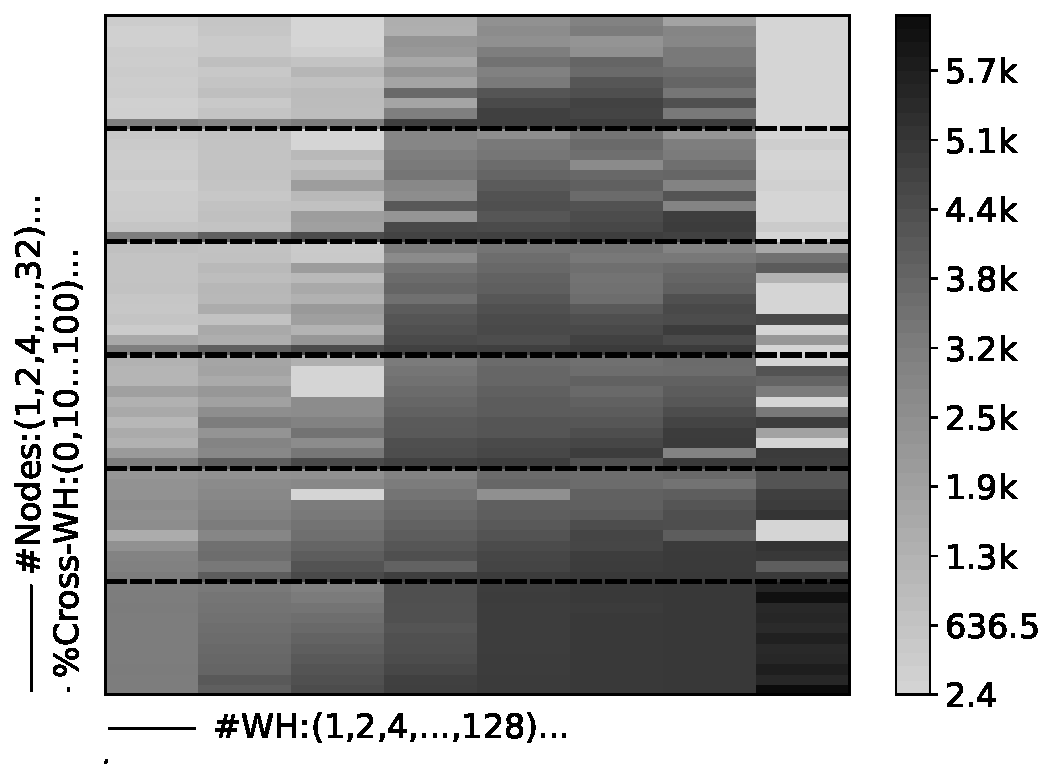
\includegraphics[width=\textwidth]{fig/calvin/Calvin_tpcc.pdf}
         \caption{Per core throughput of Calvin TPC-C.}
         \label{fig:calvin-throughput}
     \end{subfigure}
     %~
     %begin{subfigure}[t]{0.45\textwidth}
     %    \centering
     %    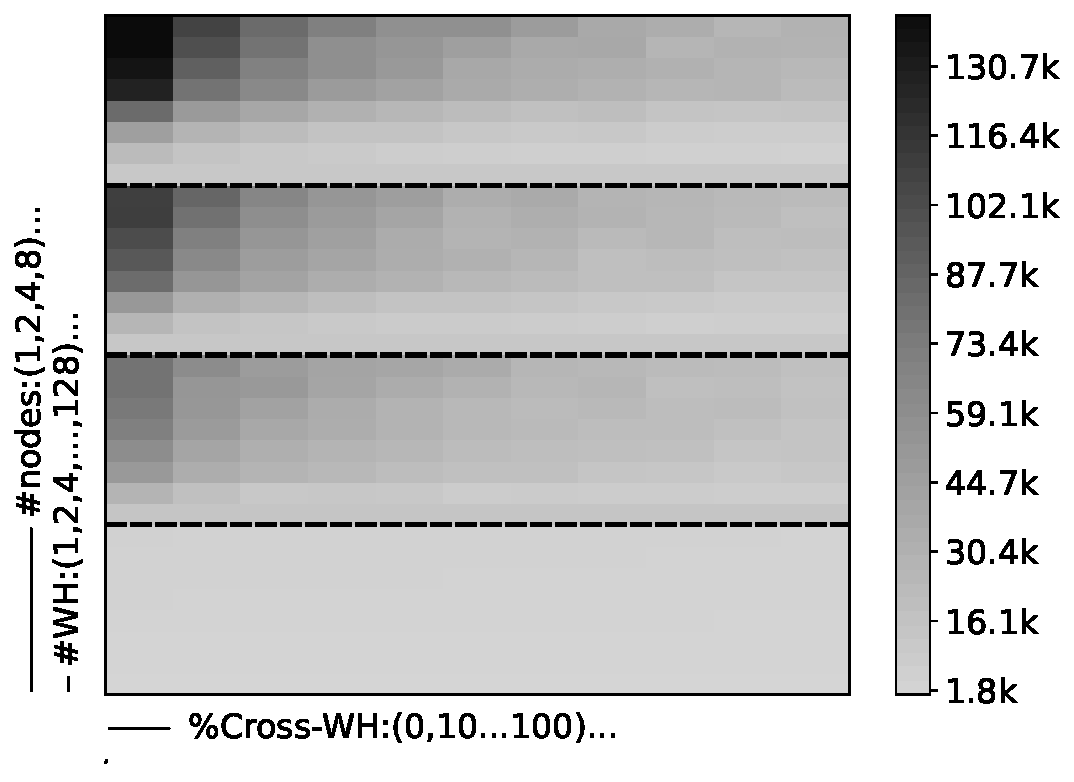
\includegraphics[width=\textwidth]{fig/aria/Calvin2-distributed-tpcc.pdf}
     %    \caption{Per core throughput of Calvin-2 from Aria TPC-C.}
     %    \label{fig:calvin2-throughput}
     %\end{subfigure}
     
     \caption{Systems with stable and unstable performance (white X indicates settings we canot run).}
     \vspace{-.1in}
     \label{fig:stable}
\end{figure*}

\vspace{-.1in}
\paragraph{Buggy or Incomplete Implementation.}

A few other issues are caused by bugs or incomplete implementation.
Due to the well-known difficulty of debugging non-deterministic issues,
we have not been able to diagnose the root cause of all of them, and
we report what we find.

\begin{itemize} [leftmargin=*]

    \vspace{-.05in}
    \item Segmentation fault. In Calvin, we find a number of settings cause
    abnormally low throughput, which further causes the bad prediction accuracy as
    shown in Section~\ref{sec:regression}. Our investigation shows these settings cause
    a segmentation fault in the middle, but the experiments still calculate the throughput
    by dividing the number of finished transactions by the total experiment time, which
    results in very low throughput. We further investigate the reason for the segmentation
    fault and find it is caused by the inappropriate handling of NULL value returned
    by set lookup, which is more likely to happen under certain settings. We are able
    to fix this issue to avoid segmentation fault but we find our fix leads to other problems.
    Since we cannot find an easy fix and Aria has already implemented a more predictable version of Calvin,
    we finally give up fixing the original version of Calvin.

    \vspace{-.05in}
   \item Lock implementation. Silo implements a competitor called PartitionedStore as
    a comparison. When testing PartitionedStore with more settings, we find the experiments
    cannot finish under certain settings. Our investigation finally traces the problem to the
    customized lock implementation of PartitionedStore: sometimes a thread cannot acquire a lock even if the
    previous owner has released the lock. We are not able to fully locate the root cause but
    we find this problem is highly likely to be correlated with the data alignment in PartitionedStore:
    this problem only happens under settings whose total size of locks is a multiple of page size,
    and by artificially adding a few bytes, we can see the problem does not happen anymore.

	\vspace{-.05in}
    \item Incomplete recovery. In TAPIR experiments we find sometimes the experiments cannot finish.
    By looking at their logs, we find these experiments trigger a timeout in the middle, probably
    due to short timeout intervals, and then trigger failure recovery. But since TAPIR does not implement
    the recovery protocol, the whole system cannot make progress. As discussed above, we enlarge the
    timeout value to avoid triggering failure recovery.
    
\end{itemize}

This type of issue is perhaps unavoidable since it is unrealistic to expect a research
prototype to be as stable and complete as a mature software and even a mature software can hardly be bug-free.
We believe the bottom line is that, by extensive evaluation, we can be aware of these issues
and have sufficient mechanisms to detect their manifestation.
Of course, if a bug frequently happens, it is better to be fixed.




\begin{figure*}[ht]
    \centering
     \begin{subfigure}[t]{0.45\textwidth}
         \centering
         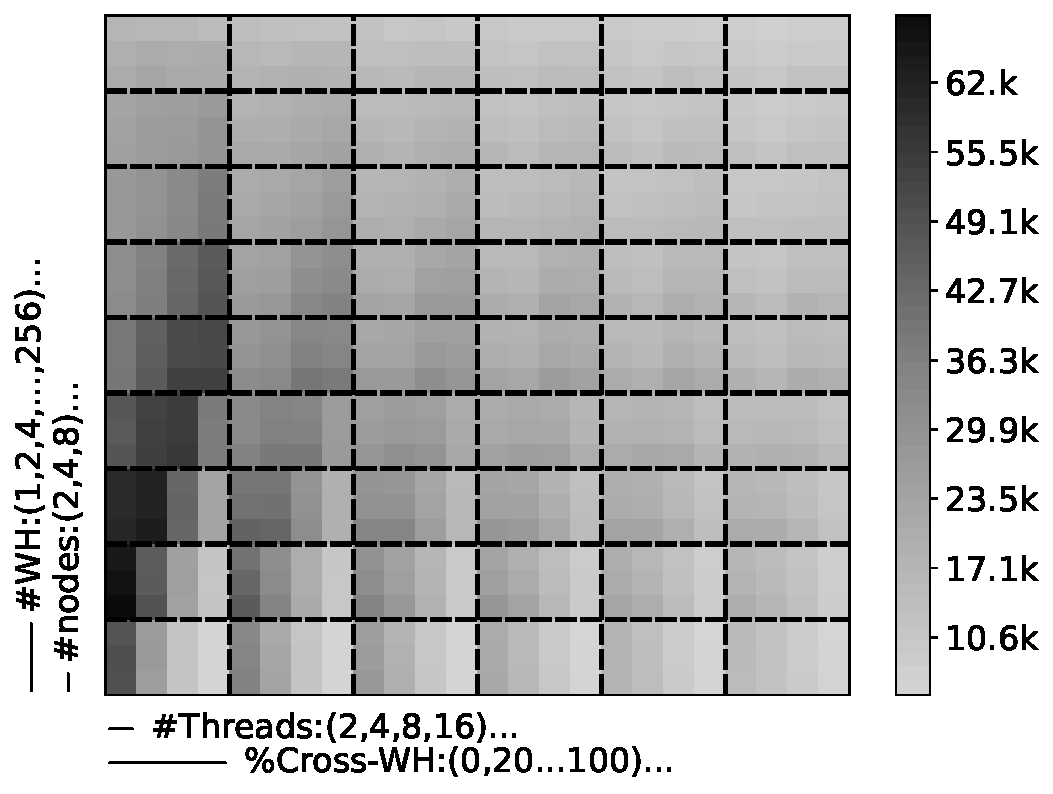
\includegraphics[width=\textwidth]{fig/drtm/drtm_tpcc.pdf}
         \caption{DrTM TPC-C throughput per server core.}
         \label{fig:drtm-throughput}
     \end{subfigure}
    ~
     \begin{subfigure}[t]{0.45\textwidth}
         \centering
         
\includegraphics[width=\textwidth]{fig/silo/silo_ycsb.pdf}
         \caption{Silo YCSB throughput per server core.}
         \label{fig:silo-ycsb-throughput}
     \end{subfigure}
     
     
     \begin{subfigure}[t]{0.45\textwidth}
         \centering
         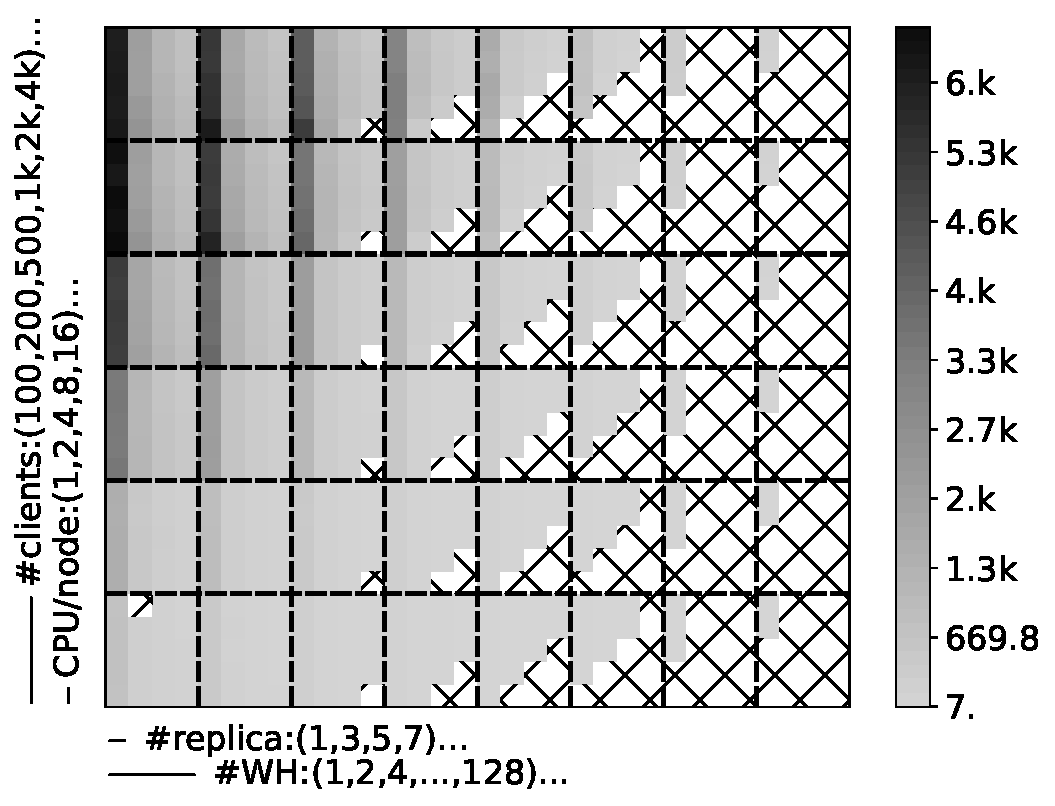
\includegraphics[width=\textwidth]{fig/janus/Janus_tpcc.pdf}
         \caption{Janus TPC-C throughput per server core.}
         \label{fig:janus-throughput}
     \end{subfigure}
     ~
     \begin{subfigure}[t]{0.45\textwidth}
         \centering
         
\includegraphics[width=\textwidth]{fig/janus/2PL_tpcc.pdf}
        \caption{2PL TPC-C throughput per server code.}
        \label{fig:2pl-throughput}
     \end{subfigure}
     
     \caption{Comprehensive analysis of system performance. White Xs indicate settings we cannot run due to resource constraints.}
     \vspace{-.1in}
     \label{fig:comprehensive}
\end{figure*}


\subsection{Comprehensive Performance Analysis and Comparison}


In this section, we present how
extensive evaluation helps to reveal performance issues
and allows a more comprehensive performance comparison.
Due to space limitation, we discuss a subset of results
here and publish all figures at our anonymous website~\cite{FigureSite}.

\vspace{-.1in}
\paragraph{Predictable vs unpredictable performance.}



As shown in Section~\ref{sec:regression}, some systems have highly predictable
performance and some are less predictable. The Tiled Heat Map can provide
a direct illustration of such problems.

As shown in Figure~\ref{fig:stable}, HERD has a very regular performance pattern:
throughput decreases with larger KVs, which is as expected; more KVs
improve the throughput by a small extent; other parameters do not seem
to have a strong impact on throughput. Aria and GAM are two other examples with
a very regular performance pattern: that's why we find it surprising
that the prediction accuracy on Aria is not good (Section~\ref{sec:regression}).

Calvin, on the other hand, has a
less regular pattern as one can see there are often abrupt throughput
changes between adjacent settings. By looking at its Tiled Heat Map, we investigate
these abnormal points, which lead to our discovery in the previous section. 
The Calvin implementation from the Aria work has a much more regular pattern.
%as shown in Figure~\ref{fig:calvin2-throughput}.




\vspace{-.1in}
\paragraph{A Comprehensive Understanding of System Performance.}



Extensive evaluation with the Tiled Heat Graph
has helped to reveal performance characteristics in a more comprehensive manner and
some of them are potential design issues.

Figure~\ref{fig:drtm-throughput} shows the throughput of DrTM, which reveals
several patterns: in general, more distributed transactions lead to lower
throughput per core, which is expected; the number of nodes does not have a
strong impact on throughput per core, which shows DrTM has good scalability
by adding more nodes; the number of warehouses and the number of threads combined
create the step-like pattern, because more threads than warehouses will create
a high contention, which results in lower throughput. However, apart from all these
explainable patterns, we find one pattern hard to explain: further increasing the
number of warehouses beyond the number of threads causes a quite significant drop
of throughput per core.
We use \emph{perf}~\cite{perf} to profile DrTM and find, with more warehouses,
DrTM spends more time on indexing. This is because DrTM uses tree indexes, and
with more data, the trees grow taller and require more time for updating and searching.

Silo has exactly the same issue as shown in Figure~\ref{fig:silo-ycsb-throughput}:
it uses Masstree as the index and since the tree grows taller with more KVs, tree update
takes longer, which causes performance degradation with more KVs.

A classic solution to this problem is to shard the data and use an index for each
shard~\cite{Decandia07Dynamo,chang06bigtable,Lee2021ShardManager}. Actually among the systems we tested,
HERD, Star, and even Silo's competitor PartitionedStore perform data partition as well.
These examples show the risk without extensive evaluation:
if a later work needs to compare with DrTM or Silo under a setting with more KVs,
its author has to optimize the prior work for a fair comparison; even worse,
if its author is unaware of these issues, s/he may make an unfair comparison.
Later we will show how this issue affects the comparison between Silo and
its competitor PartitionedStore.


%We make two comments: 1) sharding in some cases is not as straightforward as
%just partitioning data, since the system may need to handle range queries,
%load balancing across shards, etc. For such systems, the overhead of
%indexing may change the bottleneck of the system. 2) obviously it is not
%fair to compare systems using and not using sharding.

%As shown in Figure~\ref{fig:gam-throughput}, GAM has a similar pattern that
%it reaches the highest throughput with 8-16 warehouses and the throughput decreases
%with more warehouses. The reason is that GAM heavily relies on caching for
%best performance: when there are many warehouses,
%cache becomes less effective since TPC-C is dominated by random accesses.
%We don't know a good solution for this problem, but on the other hand, it may not be
%a good idea to evaluate a cache system with a random workload in the first place.

Figure~\ref{fig:janus-throughput} and Figure~\ref{fig:2pl-throughput} show the throughput of Janus
and its competitor two-phase locking (2PL). They have the configuration
constraint that $\#CPUsPerNode \times \#Nodes = \#replica \times \#WH$.
In other words, increasing \#WH will increase the number of nodes in these figures.
As shown in Figure~\ref{fig:janus-throughput}, Janus' per-core throughput grows
with more clients since too few clients will not be able to saturate the server;
its per-core throughput drops with more replicas, which is expected since more
replicas will incur more messages; its per-core throughput keeps stable when
adding more CPUs per node, which means it scales up quite well; however, when
adding nodes (i.e., warehouses), we can see its per-core throughput drops to some degree, which
means it does not scale out very well. We investigate these
experiments but do not find a clear bottleneck and we suspect the performance drop
is caused by Janus' construction of a global dependency graph, which may incur
more overhead when adding more nodes. How to improve the scalability
of a global dependency graph could be an interesting research topic.

Figure~\ref{fig:2pl-throughput} shows that 2PL has a very different pattern:
its per-core throughput drops with more replicas, which is expected and the same as
Janus; its combination of number of clients and number of warehouses shows the
step pattern, which indicates 2PL can achieve the highest throughput if its \#clients and \#WH
has a fixed rate. This is due to the fact that too few clients cannot saturate
the server and too many clients will cause many deadlocks. Finally, we observe 2PL
can both scale up and scale out pretty well, which is reasonable since 2PL has no
inherent bottleneck.

\vspace{-.1in}
\paragraph{A Comprehensive Comparison.}

\begin{figure}[t]
    \centering
    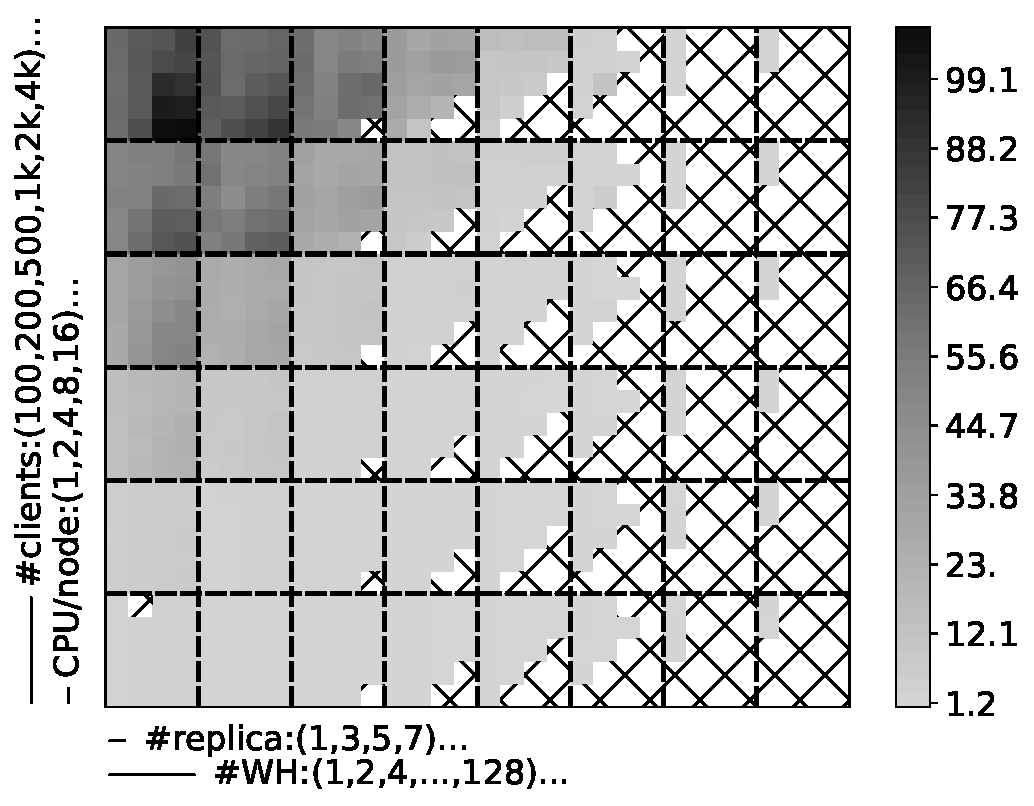
\includegraphics[width=0.45\textwidth]{fig/janus/[comp]Janus-vs-2PL_tpcc}
    \caption{Janus over 2PL. White Xs indicate settings we cannot run due to resource constraint.}
    \vspace{-.1in}
    \label{fig:janus_vs_2pl}
\end{figure}

%\begin{figure}[t]
%    \centering
%    
\includegraphics[width=0.45\textwidth]{fig/janus/2PL_tpcc.pdf}
%    \caption{Throughput of 2PL}
%    \label{fig:2pl}
%\end{figure}

\begin{figure}[t]
    \centering
    
\includegraphics[width=0.45\textwidth]{fig/silo/[comp]Silo-vs-PartitionedStore_tpcc}
    \caption{Silo over PartitionedStore}
    \vspace{-.1in}
    \label{fig:silo-vs-partitionedstore}
\end{figure}

Finally, we use two examples to show how extensive evaluation can allow
a more comprehensive evaluation. To compare two works A and B, we use the Tiled
Heat Map to draw throughput of A over throughput of B.

Figure~\ref{fig:janus_vs_2pl} shows the comparison between Janus and 2PL. As one can
see, Janus can achieve the highest improvement on the top left corner (i.e, more clients
and fewer warehouses), which incurs the highest contention level; its improvement
decreases with more warehouses, because as discussed above, Janus does not scale out
very well but 2PL does. It would be interesting to see the trend in a large setting
but unfortunately
we do not have enough machines for that.

%\begin{figure}[t]
%    \centering
%    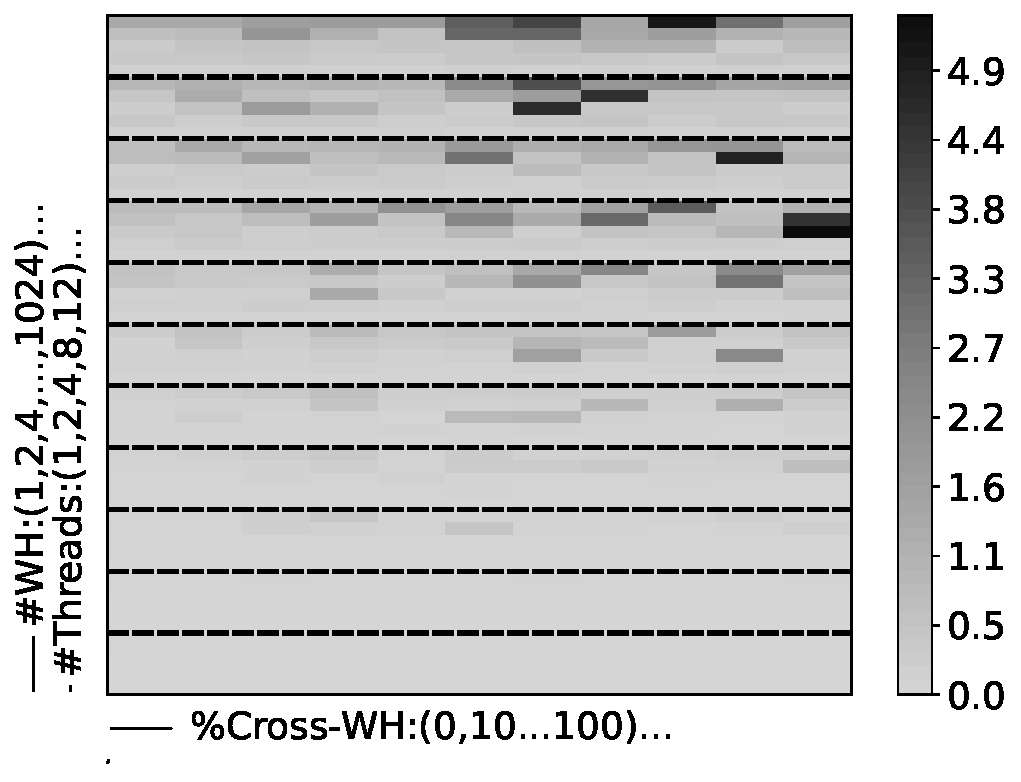
\includegraphics[width=0.45\textwidth]{fig/aria/[comp]aria-vs-Pwv_tpcc}
%    \caption{Aria over Pwv}
%    \label{fig:aria-vs-pwv}
%\end{figure}

%\begin{figure}[t]
%    \centering
%    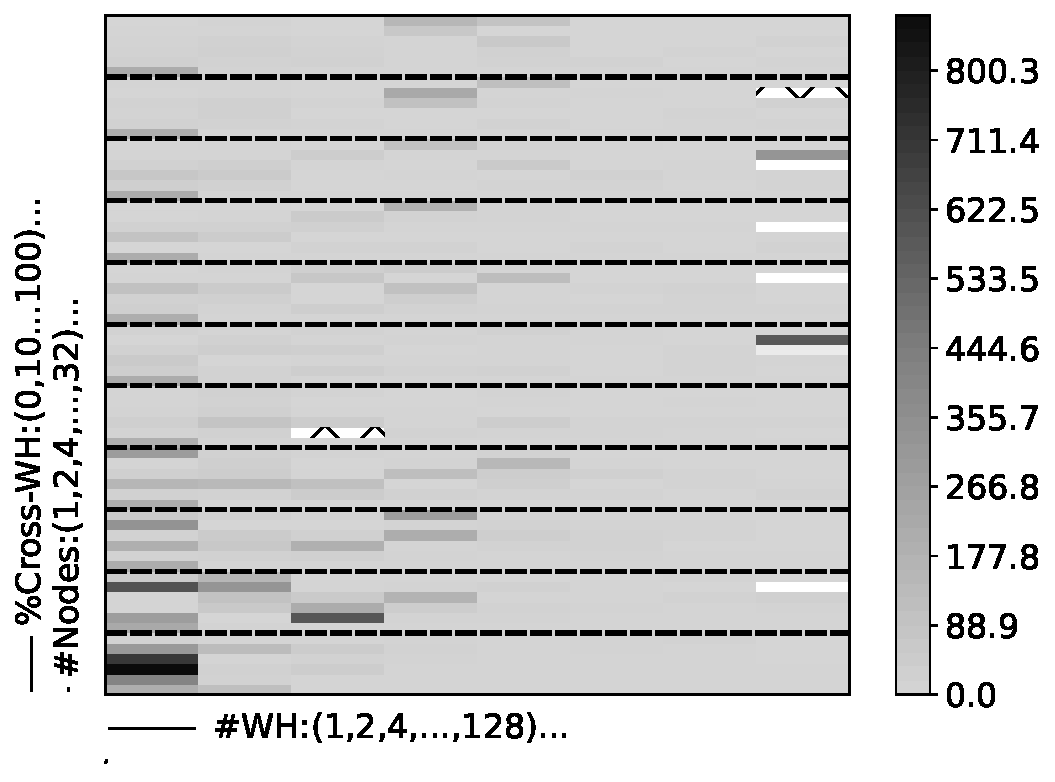
\includegraphics[width=0.45\textwidth]{fig/calvin/[comp]Calvin-vs-2pl_tpcc}
%    \caption{Calvin over 2PL}
%    \label{fig:calvin-vs-2pl}
%\end{figure}

%\begin{figure}[t]
%    \centering
%    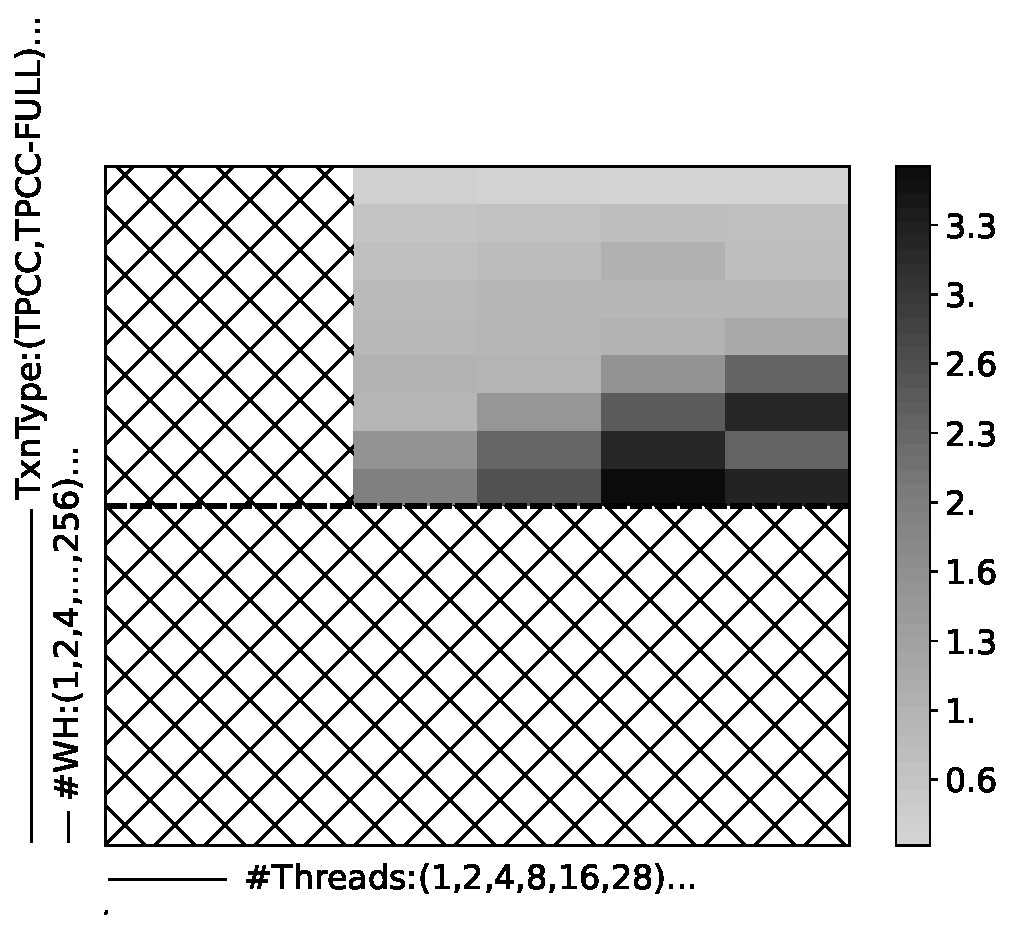
\includegraphics[width=0.45\textwidth]{fig/cicada/[comp]cicada-vs-MOCC_tpcc}
%    \caption{Cicada over MOCC}
%    \label{fig:cicada-vs-MOCC}
%\end{figure}




Figure~\ref{fig:silo-vs-partitionedstore} shows the comparison between
Silo and its competitor PartitionedStore. In general, we can see the improvement drops with more
warehouses, fewer threads, and fewer cross-warehouse transactions. Our analysis shows two reasons.
First, Silo targets addressing contentions and contention level decreases with more
warehouses, fewer threads, and fewer cross-warehouse transactions, so Silo's relative
benefit becomes smaller. Second, as mentioned above, Silo does not partition data so
its tree index grows taller with more data; PartitionedStore partitions data and thus
does not have this problem. Among these two reasons, the first reason is the one we are
interested in since Silo targets addressing contentions; the second one does not seem
to be a fundamental limitation of Silo and is diminishing the true improvement of Silo.

\vspace{-.1in}
\paragraph{Memory consumption.}
From the extensive evaluation, we observe the memory consumption of these
systems vary a lot. We measure the memory consumption
per warehouse under the TPC-C workload: for systems that perform customized
memory allocation, we set a maximal memory limit
and then increase the number of warehouses, till the system crashes; for systems
relying on malloc, we use the \emph{sysinfo} call to get memory consumption
before and after loading a warehouse. Our measurement shows that 
their per-warehouse memory consumption varies significantly: 33MB for Calvin, 59MB for Aria, 64MB for Star and DrTM,
330MB for Silo, 360MB for Cicada, and over 600MB for GAM.
Such gap
is caused by the difference among their exact data to populate, their
data layouts, and their index formats.

For in-memory systems, memory consumption is certainly an important factor and
we suggest to at least report the memory consumption numbers. Of course how
to reduce memory consumption can be a research topic as well.


\vspace{-.1in}
\paragraph{Effects of Extensive Evaluation.}
Most of the issues discussed in this section are not obvious in the original
settings of their corresponding papers: DrTM assumes the number of threads
is equal to the number of warehouses and tests with at most 28 warehouses,
Silo uses a fixed 160M key-value pairs in YCSB and uses at most 32 warehouses
in TPC-C. Therefore, for these two systems, the trend that
more data lead to performance degradation is unclear. Janus tests with 6 warehouses,
so the scalability issue is unclear as well.
Extensive evaluation and proper visualization can help to reveal these problems
and facilitate future comparison.


